% fig10-data-ownership.tex — Figure 10: Data ownership (DEV-GOV-03)
%
% Who may write each fact, and who may only read it. The rule the picture encodes
% is single-writer plus read-only references: no fact in this system has two
% writers, and no cross-domain reader is also a writer.
\documentclass[tikz,border=10pt]{standalone}
\usetikzlibrary{arrows.meta,positioning,fit,backgrounds,calc}

\begin{document}
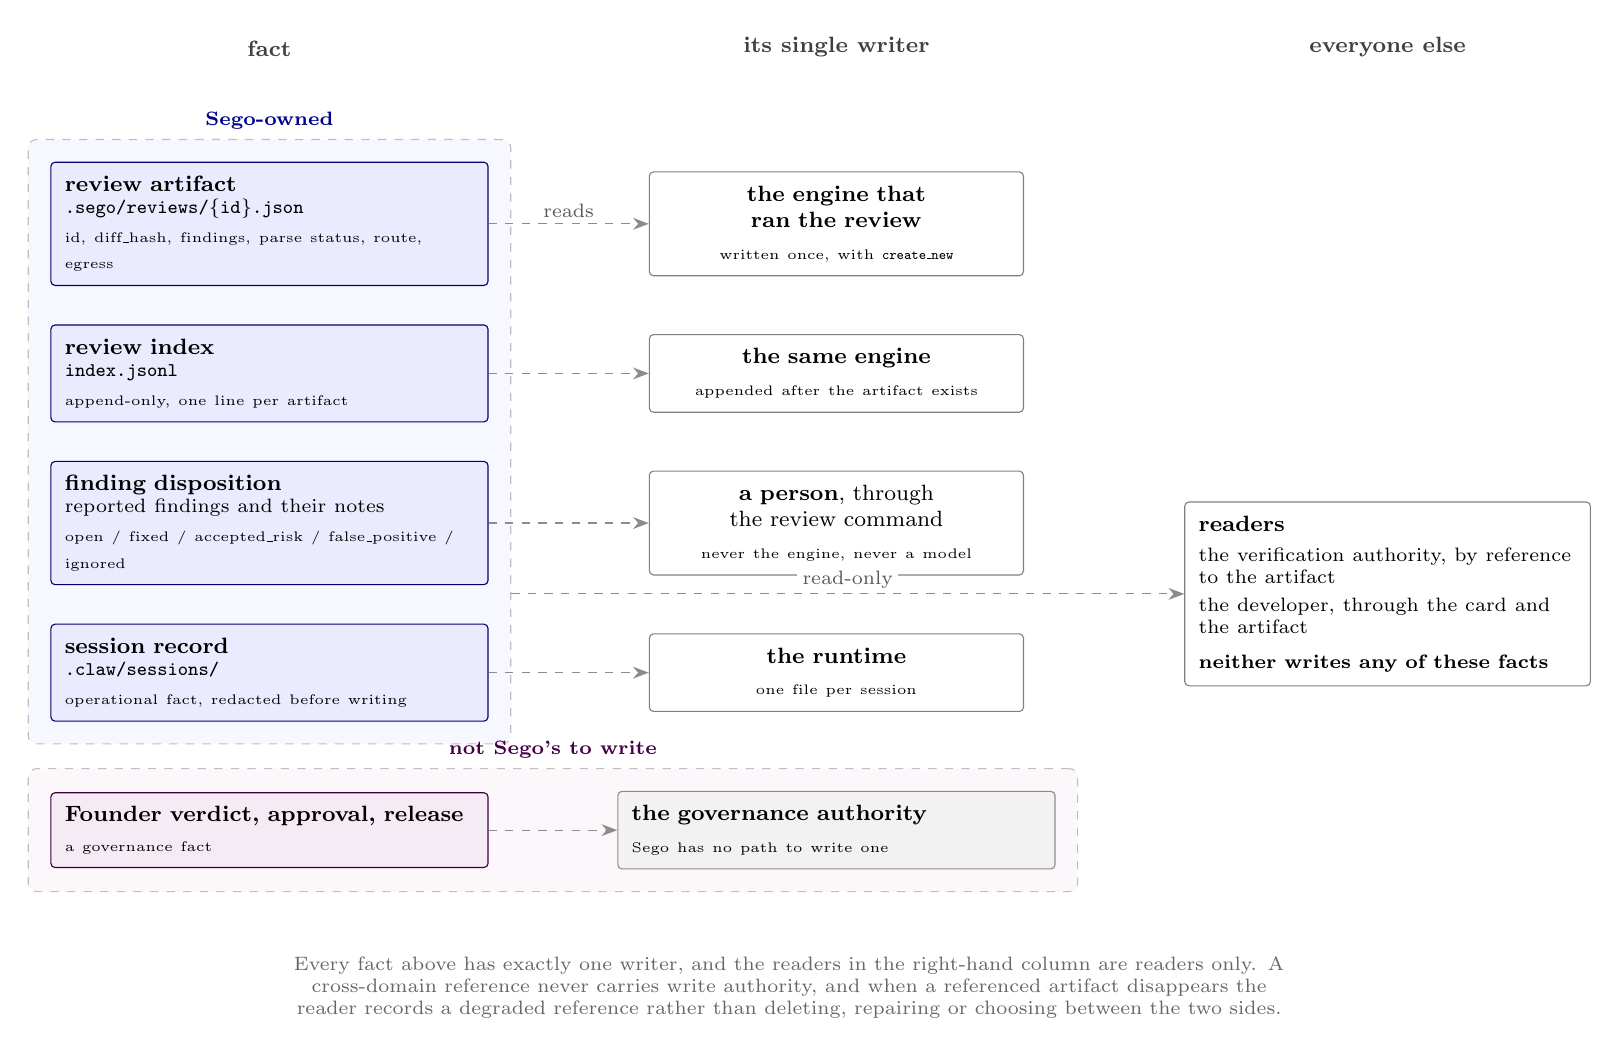
\begin{tikzpicture}[
  x=1cm, y=1cm,
  font=\small,
  fact/.style={draw, rounded corners=1.5pt, fill=white, draw=black!50,
               font=\footnotesize, align=left, inner sep=5pt, text width=52mm},
  mine/.style={fact, fill=blue!8, draw=blue!45!black},
  theirs/.style={fact, fill=violet!8, draw=violet!45!black},
  outside/.style={fact, fill=black!5, draw=black!45},
  arr/.style={-{Stealth[length=2.2mm]}, thick, draw=black!70},
  ro/.style={-{Stealth[length=2mm]}, draw=black!45, dashed},
  lab/.style={font=\scriptsize, text=black!65, inner sep=2pt, fill=white},
  hdr/.style={font=\footnotesize\bfseries, text=black!75, anchor=south},
  grp/.style={draw=black!25, dashed, rounded corners=3pt, inner sep=8pt}
]

% ---------------- columns ----------------
\node[hdr] at (-6.6, 3.5) {fact};
\node[hdr] at (0.6, 3.5) {its single writer};
\node[hdr] at (7.6, 3.5) {everyone else};

% ---------------- Sego-owned facts ----------------
\node[mine] (art) at (-6.6, 1.5)
  {\textbf{review artifact}\\ \scriptsize \texttt{.sego/reviews/\{id\}.json}\\[1pt]
   \tiny id, diff\_hash, findings, parse status, route, egress};
\node[fact, font=\footnotesize, align=center, text width=44mm] (artw) at (0.6, 1.5)
  {\textbf{the engine that ran the review}\\[2pt] \tiny written once, with \texttt{create\_new}};

\node[mine] (idx) at (-6.6, -0.4)
  {\textbf{review index}\\ \scriptsize \texttt{index.jsonl}\\[1pt]
   \tiny append-only, one line per artifact};
\node[fact, font=\footnotesize, align=center, text width=44mm] (idxw) at (0.6, -0.4)
  {\textbf{the same engine}\\[2pt] \tiny appended after the artifact exists};

\node[mine] (disp) at (-6.6, -2.3)
  {\textbf{finding disposition}\\ \scriptsize reported findings and their notes\\[1pt]
   \tiny open / fixed / accepted\_risk / false\_positive / ignored};
\node[fact, font=\footnotesize, align=center, text width=44mm] (dispw) at (0.6, -2.3)
  {\textbf{a person}, through the review command\\[2pt] \tiny never the engine, never a model};

\node[mine] (sess) at (-6.6, -4.2)
  {\textbf{session record}\\ \scriptsize \texttt{.claw/sessions/}\\[1pt]
   \tiny operational fact, redacted before writing};
\node[fact, font=\footnotesize, align=center, text width=44mm] (sessw) at (0.6, -4.2)
  {\textbf{the runtime}\\[2pt] \tiny one file per session};

% ---------------- not Sego's to write ----------------
\node[theirs] (verdict) at (-6.6, -6.2)
  {\textbf{Founder verdict, approval, release}\\[1pt]
   \tiny a governance fact};
\node[outside] (verdictw) at (0.6, -6.2)
  {\textbf{the governance authority}\\[2pt] \tiny Sego has no path to write one};

\begin{scope}[on background layer]
  \node[grp, fill=blue!3, label={[font=\scriptsize\bfseries, text=blue!55!black]above:Sego-owned}]
    (segofacts) [fit=(art)(idx)(disp)(sess)] {};
  \node[grp, fill=violet!3, label={[font=\scriptsize\bfseries, text=violet!55!black]above:not Sego's to write}]
    (govfacts) [fit=(verdict)(verdictw)] {};
\end{scope}

% ---------------- read-only arrows ----------------
\draw[ro] (art.east) -- node[lab, above] {reads} (artw.west |- art);
\draw[ro] (idx.east) -- (idxw.west |- idx);
\draw[ro] (disp.east) -- (dispw.west |- disp);
\draw[ro] (sess.east) -- (sessw.west |- sess);
\draw[ro] (verdict.east) -- (verdictw.west |- verdict);

% ---------------- cross-domain reads ----------------
% One box rather than one per fact. Per-fact reader boxes put a dashed arrow
% through the writer column for every row, which read as if the writers did the
% reading.
\node[fact, fill=white, draw=black!50, text width=48mm, font=\footnotesize, align=left] (readers) at (7.6, -3.2)
  {\textbf{readers}\\[3pt] \scriptsize the verification authority, by reference to the artifact\\[2pt]
   \scriptsize the developer, through the card and the artifact\\[3pt]
   \textbf{\scriptsize neither writes any of these facts}};

% Routed through the gap between two writer boxes. A horizontal arrow at the
% readers' own height would cross a writer box and print its label on top of it.
\draw[ro] (segofacts.east |- readers.west) -- node[lab, above] {read-only} (readers.west);

\node[font=\scriptsize, text=black!60, text width=184mm, align=center] at (0, -8.2)
  {Every fact above has exactly one writer, and the readers in the right-hand column are readers only. A cross-domain reference
   never carries write authority, and when a referenced artifact disappears the reader records a degraded reference rather than
   deleting, repairing or choosing between the two sides.};

\end{tikzpicture}
\end{document}
